\section{Laplacetransformation}

Laplacetransformationen werden für kausale Funktionen $f(t)$ definiert, für die gilt $f(t) = 0$ für $t < 0$

\vspace{0.1cm}

Es gilt die Korrespondenz: $f(t) \; \laplace \; F(s)$ (Bildbereich)

\vspace{0.1cm}

\textbf{Hinweis:} Eine Funktion kann kausal gemacht werden, indem man sie mit der Einheitssprungfunktion $\sigma(t)$ multipliziert.


\subsection{Berechnung (einseitige) Laplacetransformation}

\renewcommand{\arraystretch}{1.8}
\begin{tabular}{ll}
    Transformation:     & $F(s) = \mathcal{L} \{ f(t) \} := \int \limits_0^{\infty} f(t) \cdot \e^{-s \, t} \, \diff t$ \quad mit $s = \rho + \jimg \omega$   \\
    Rücktransformation: & \textrightarrow\ Tabellen und Tipps verwenden! 
\end{tabular}
\renewcommand{\arraystretch}{1}


\subsection{Konvergenzhalbebene}

Es gibt jeweils mehrere (komplexe) Zahlen $s$, \textbf{für welche das Laplace-Integral konvergiert.} 
Die Konvergenzhalbebene beinhaltet alle diese Zahlen $s$

\begin{minipage}[c]{0.48\columnwidth}
    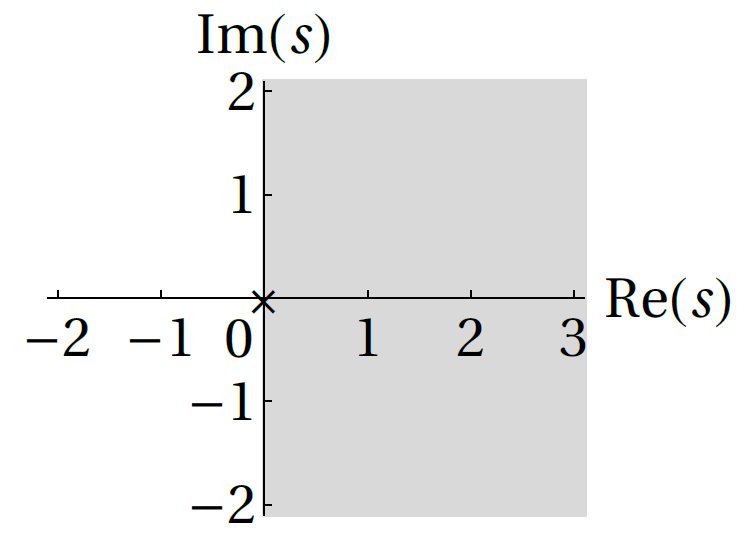
\includegraphics[width=\columnwidth]{images/konvergenzhalbebene} 
\end{minipage}
\hfill
\begin{minipage}[c]{0.48\columnwidth}
    Die Halbebene wird durch die \textbf{am weitesten rechts liegende Polstelle} von $F(s)$ begrenzt (Kreuzchen)
    \vspace{0.2cm}
    Falls $F(s)$ keine Polstelle hat, ist die Konvergenzhalbebene gleich $\mathbb{C}$
\end{minipage}


Liegt die imaginäre Achse in der Konvergenzhalbebene, so \textbf{existiert} die Fouriertransformierte!

\textrightarrow\ Man erhält sie, indem man $s$ durch $\jimg \omega$ ersetzt


\example{Berechnung der Laplacetransformation}

$f(t) = \begin{cases}			
    0           & \text{für} \; t < 0 \\
    \frac{1}{2} & \text{für} \; t = 0 \\ 
    e^{at}      & \text{für} \; t > 0 
\end{cases}$  \quad  mit $a \in \mathbb{R}$

\begin{align*}
    F(s)    &= \int \limits_0^{\infty} \e^{at} \, \e^{-st} \, \diff t = \int \limits_0^{\infty} \e^{-(s-a)t} \, \diff t = - \frac{1}{s-a} \e^{-(s-a)t} \biggr|_0^{\infty} \\
            &= - \frac{1}{s-a} \left( \lim \limits_{t \to \infty} \e^{-(s-a)t} -1 \right) = - \frac{1}{s-a} \left( \lim \limits_{t \to\infty} \e^{-((\rho+ \jimg \omega)-a)t} -1 \right) \\
            &= - \frac{1}{s-a} \left( \lim \limits_{t \to \infty} \e^{-(\rho-a)t} \, \e^{- \jimg \omega t} -1 \right)
\end{align*}

\textrightarrow\ Überlegen, was mit welchem Teil passiert! 

\vspace{0.2cm}

\begin{tabular}{ll}
    $\e^{- j \omega t}$ & Zahl auf Einheitskreis (Betrag 1) \\
    $\e^{-(\rho - a)t}$ & $\rho > a$ \quad \textcolor{blue}{Konvergenz gegen 0} \\
                        & $\rho = a$ \quad Konvergenz gegen 1 \\
                        & $\rho < a$ \quad Divergenz \\
\end{tabular}

\vspace{0.2cm}
$$ F(s) = ... = - \frac{1}{s-a} \left( \lim \limits_{t \to \infty} \e^{-(s-a)t} -1 \right) = \frac{1}{s-a} \text{ für } \rho = \Re(s) > a $$

$$ \text{ \textrightarrow\ Korrespondenzpaar: } \e^{at} \; \laplace \; \frac{1}{s-a} $$


\subsection{Tipps zu Rücktransformationen}

\begin{itemize}
    \item Zähler und Nenner gleichgradig \textrightarrow\ Polynomdivision
    \item Zusammengesetzte Nennerfunktion \textrightarrow\ PBZ
    \item Nenner \textbf{keine} reelle NS \textrightarrow\ Ansatz $ \sin(\omega t), \, \cos(\omega t)$
    \item Nenner hat reelle NS \textrightarrow\ Ansatz \textbf{nicht} $\sin(\omega t), \, \cos(\omega t)$
\end{itemize}


\subsection{Lineare DGL mittels Laplacetransformation lösen}

\subsubsection{Vorgehen: Lösen einer DGL mit Laplace}

\begin{enumerate}
    \item DGL inkl. Störfunktion $f(t)$ in Bildbereich transformieren \\
        \textrightarrow\ Anfangswerte für $f^{(n)}(0^+)$ einsetzen!
    \item Gleichung nach Laplace-Transofrmierter der gesuchten Funktion umformen
    \item Rücktransformation in den Zeitbereich
\end{enumerate}


\example{Lösung einer DGL mit Laplace}

\begin{minipage}[c]{0.6\columnwidth}
    \begin{tabular}{ll}
        DGL:            & $\ddot{y}(t) + 2 \, \dot{y}(t) + 5 \, y(t) = f(t)$ \\
        Anfangswerte:   & $y(0) = 0$; \quad $\dot{y}(0) = 0$
    \end{tabular}
\end{minipage}
\hfill
\begin{minipage}[c]{0.35\columnwidth}
    \textrightarrow\ Finde $y(t)$
\end{minipage}

\vspace{0.2cm}

\begin{enumerate}
    \setlength\itemsep{3pt}
    \item $\laplace \; s^2 \cdot Y(s) - s \cdot 0 - 0 + 2( s \cdot Y(s) - 0) + 5 \cdot Y(s) = 1(s)$ \\
        $s^2 \cdot Y(s)+ 2 \cdot s \cdot Y(s) + 5 \cdot Y(s) = 1(s)$
    \item $Y(s) = \frac{1}{s^2 + 2s +5}$
    \item Rücktransformation mit Tabellen
\end{enumerate}


\subsection[Übertragungsfunktion (LTI-Systeme)]{Übertragungsfunktion $\bm{G(s)}$ (LTI-Systeme)}

\begin{minipage}[c]{0.4\columnwidth}
    $$ G(s) = Y_{\delta}(s) = \frac{Y(s)}{X(s)} $$
\end{minipage}
\hfill
\begin{minipage}[c]{0.58\columnwidth}
    \begin{tabular}{ll}
        Eingangssignal: & $x(t) \; \laplace \; X(s)$    \\
        Ausgangssignal: & $y(t) \; \laplace \; Y(s)$
    \end{tabular}
\end{minipage}

\begin{center}
    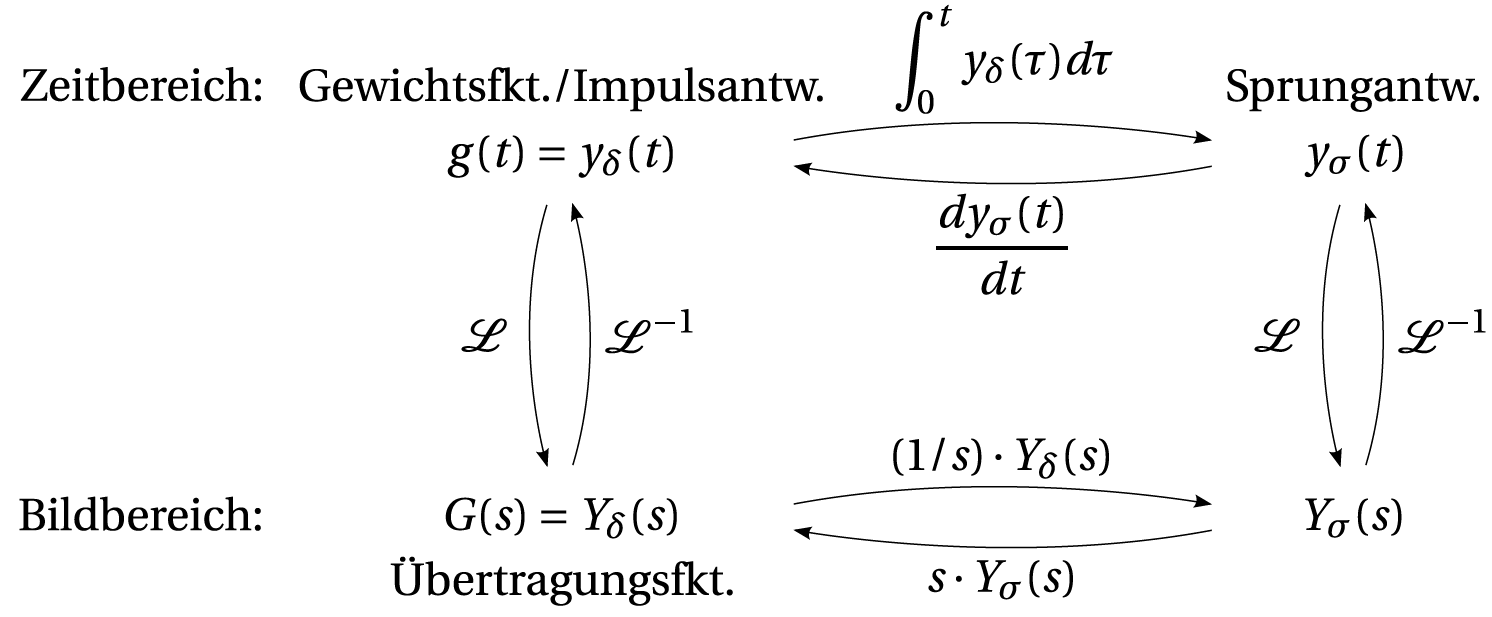
\includegraphics[width=0.75\columnwidth]{images/impulsantwort_uebertragungsfunktion.png} 
\end{center}


\subsubsection{Übertragungsfunktion $\bm{G(s)}$ aus DGL bestimmen}

\begin{tabular}{ll}
    DGL:    & $\sum \limits_{k=0}^{n} a_k \cdot y^{(k)} (t) = f(t) = \sum \limits_{k=0}^{m} b_k \cdot x^{(k)} (t)$ \\
    UTF:    & $G(s) = \frac{q(s)}{p(s)} = \frac{\sum \limits_{k=0}^{m} b_k \cdot s^k}{\sum \limits_{k=0}^{n} a_k \cdot s^k}$ 
\end{tabular}

$$ \underrightarrow{f(t) = x(t)} \quad G(s) = \frac{1}{p(s)} = \frac{1}{\sum \limits_{k=0}^{n} a_k \cdot s^k} = \frac{1}{\text{char. \; Polynom}} $$



\subsection[Übertragungsfunktion -- Frequenzgang]{Übertragungsfunktion $\bm{G(s)}$ \textrightarrow\ Frequenzgang $\bm{H(\omega)}$}

Wenn die Konvergenzhalbebene einer Übertragungsfunktion $G(s)$ eines LTI-Systems die \textbf{imaginäre Achse beinhaltet}, so gilt:

$$ H(\omega) = G(j \omega) = G(s) \biggr|_{s = j \omega} \qquad \text{\textrightarrow\ in $G(s)$ alle $s$ durch $\jimg \omega$ ersetzen} $$


\subsection{BIBO-Stabilität}

Ein LTI-System ist BIBO-stabil, wenn ein \textbf{beschränktes Eingangssignal} $x(t)$ zu einem \textbf{beschränkten Ausgangssignal} $y(t)$
mit $\mathrm{max}( \vert y(t) \vert) < \infty$ führt.


\subsubsection{Zeitbereich}

Ein LTI-System ist BIBO-stabil, wenn die Impulsantwort \textbf{absolut integrierbar} ist:
$$ \int \limits_{- \infty}^{\infty} \vert y_{\delta} (t) \vert \, \diff t = \int \limits_{-\infty}^{\infty} \vert g(t) \vert \, \diff t < \infty $$


\subsubsection{Bildbereich}

Ein LTI-System ist BIBO-stabil, wenn  die \textbf{Konvergenzhalbebene} der Übertragungsfuntion $G(s)$ die \textbf{imaginäre Achse enthält}

\textrightarrow\ $\Re(s_p) < 0$ bzw. Realteil der Polstelle $< 0$


\subsection{Pol-Nullstellen Plan (PN-Plan)}

Der PN-Plan stellt die Polstellen und Nullstellen einer Übertragungsfunktion $G(s)$ eines LTI-Systems in der \textbf{komplexen Zahlenebene} dar.

\vspace{0.2cm}

\begin{tabular}{ll}
    Nullstellen:    & als Kreise dargestellt    \\
    Polstellen:     & als Kreuzchen dargestellt 
\end{tabular}


\subsection{Zusammengesetzte LTI-Systeme}

\begin{tabular}{ccc}
    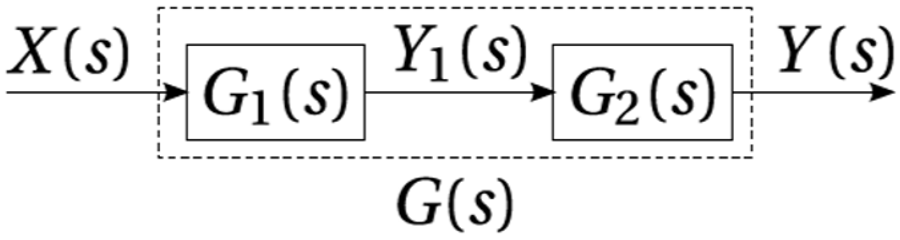
\includegraphics[width=3.5cm]{images/zusammengesetzte_LTI-systeme_a.png}    & & 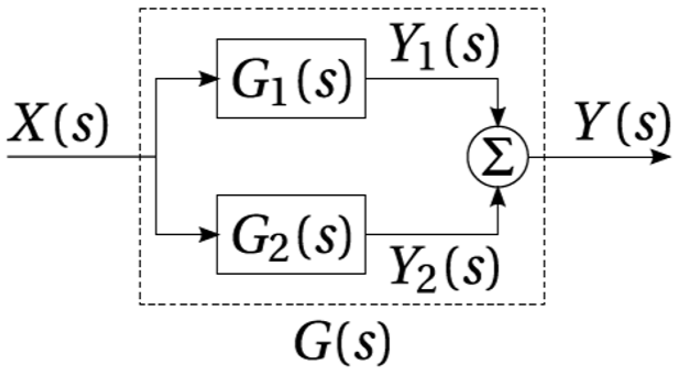
\includegraphics[width=3.5cm]{images/zusammengesetzte_LTI-systeme_b.png}    \\
    $G(s) = G_1(s) \cdot G_2(s)$                                                & & $G(s) = G_1(s) + G_2(s)$                                                    \\
    \\
    \\
    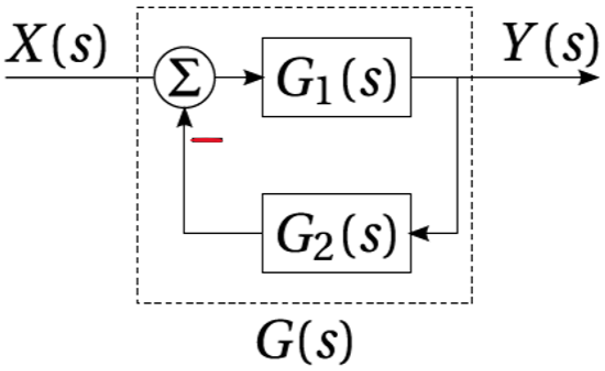
\includegraphics[width=3.5cm]{images/zusammengesetzte_LTI-systeme_c.png}    & & 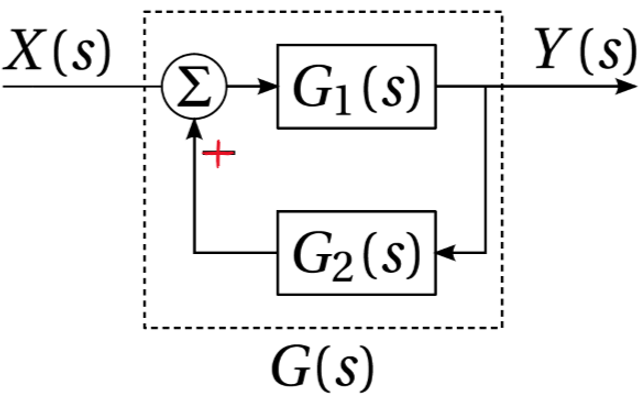
\includegraphics[width=4cm]{images/zusammengesetzte_LTI-systeme_d.png}      \\
    $G(s) = \frac{G_1(s)}{1 + G_1(s) \cdot G_2(s)}$                             & & $G(s) = \frac{G_1(s)}{1 - G_1(s) \cdot G_2(s)}$
\end{tabular}

